
%\hypertarget{aula-4}{%
%\chapter{Aula: 4}\label{aula-4}}




\hypertarget{processos-e-threads}{%
\chapter{Processos e threads}\label{processos-e-threads}}

\hypertarget{thread-uxe9-uma-parte-do-processo}{%
\subsection{Thread é uma parte do Processo}\label{thread-uxe9-uma-parte-do-processo}}

Como dito na aula anterior, um processo é uma entidade ativa a qual se
refere à um programa em execução. Porém, a CPU não recebe essa entidade
na sua integralidade para processamento, e sim uma parte da mesma
chamada de \emph{Thread} (a \emph{Thread} pode ser definida como uma
unidade de processamento do processo). Nessa está contido os elementos
necessários para a mudança de contexto da CPU (\emph{CPU Context
Switch}), como os valores dos registradores utilizados, a memória Stack
e o PC (\emph{Program Counter}).

Em sistemas \emph{single-threaded} (única \emph{thread} por processo,
normalmente encontrado em sistemas mais antigos), cada nova tarefa a ser
executada deve-se passar pela criação de um novo processo.

\hypertarget{concurrency-vs-parallelism}{%
\subsection{Concurrency vs Parallelism}\label{concurrency-vs-parallelism}}

Uma observação importante é que um programa, em um sistema com um único
núcleo de processamento, pode rodar em simultâneo (\emph{concurrency})
com outros programas, devido a alternação do processo a ser executado
pela CPU em certos períodos de tempo, porém não em paralelo
(\emph{parallelism}), por não ter múltiplos núcleos.

\hypertarget{concurrency}{%
\subsection{Concurrency}\label{concurrency}}

Os processos são distribuídos para a CPU com a técnica
\emph{Round-Robin}, com a qual é gerada uma fila de processos, e a saída
de cada fila vai para o processador. Após um certo período de tempo,
esse processamento é interrompido, o seu contexto é salvo, e o processo
volta para o final da fila (observar que há políticas de prioridades. No
exemplo está sendo considerado que todos os processos têm a mesma
prioridade). Um novo processo então é chamado para execução, com o seu
contexto de CPU sendo carregado. Essa mudança de contexto da CPU
(\emph{CPU context-switch}) é o que torna possível a CPU retomar o
processamento de um processo específico do momento que o mesmo foi
anteriormente interrompido. Esse ciclo continua até a conclusão de todos
os processos.

\hypertarget{criauxe7uxe3o-de-novos-processos}{%
\subsection{Criação de novos processos}\label{criauxe7uxe3o-de-novos-processos}}

Na linguagem C, a criação de um novo processo passa pela função
\texttt{clone(2)}, a qual copia, conforme instruções do programador,
todos os elementos do processo original para o novo processo,
consumindo, assim, recursos como a memória, com a locação múltipla dos
mesmos dados. Uma tentativa de otimização pode ser observada na função
\texttt{fork(2)} (que é uma implementação específica da função
\texttt{clone(2)}), que utiliza o conceito de \texttt{CoW} (\emph{Copy
on Write}, ou cópia na escrita, que é uma funcionalidade do sistema de
gerenciamento de memória), somente copiando os dados, para o novo
endereço de memória, caso haja alteração dos mesmos. Isso é possível com
o uso dos ponteiros, discutidos na aula anterior, para a leitura dos
dados. É importante notar que a execução do processo criado continuará a
partir da última posição do IP (\emph{Instruction Pointer}, ou ponteiro
de instrução), fazendo com que as instruções escritas antes do
\texttt{clone(2)} ou \texttt{fork(2)} nunca sejam lidas.

A função \texttt{fork()} retorna:

\begin{enumerate}
\def\labelenumi{\arabic{enumi}.}

\item
  -1, caso tenha falhado;
\item
  0, para o processo filho, com o PPID (\emph{Parent Process
  Identifier}, ou identificador do processo pai) equivalendo ao PID
  (\emph{Process Identifier}, ou identificador do processo) do processo
  pai
\item
  PID do processo filho, no processo pai.
\end{enumerate}


\begin{minted}[mathescape, linenos]{c}

    #include <stdio.h>
    #include <sys/types.h>
    #include <unistd.h>
    
    int main()
    {
            printf("Before fork: %d \n", getpid());
            pid_t returned = fork(void);
            
            if(returned == 0){
                    printf("Child here: %d \n", getpid());
            } else {
                    printf("Parent here: %d, child pid: %d \n", getpid(), returned);
            }
            
            return 0;
    }

\end{minted}



\hypertarget{por-que-devemos-criar-novos-processos}{%
\subsection{Por que devemos criar novos processos?}\label{por-que-devemos-criar-novos-processos}}

Há dois motivos para a criação de novos processos (em sistemas mais
antigos):

\begin{enumerate}
\def\labelenumi{\arabic{enumi}.}
\tightlist
\item
  Inicialização de um novo programa, com o \texttt{execve(2)}.
\item
  Múltiplas tarefas de um mesmo programa.
\end{enumerate}

Apesar da otimização citada na seção anterior (com o \texttt{CoW}), o
procedimento de criação de um novo processo é custoso de recursos
computacionais, sendo o \emph{multi-threading} (múltiplas threads no
mesmo processo) uma solução para a criação de múltiplas tarefas de um
mesmo programa (caso 2).

\hypertarget{execve2}{%
\subsection{execve(2)}\label{execve2}}

A função \texttt{execve(2)} tem como objetivo alterar a imagem de
execução, que está contida no processo, para a do novo programa, isso é,
o \emph{Data}, \emph{Heap}, \emph{Stack} e \emph{Text} serão carregados
com o conteúdo do novo programa.

A execução do programa \texttt{hello.c}, dentro do \texttt{execv.c},
ambos escritos abaixo, retornará o mesmo \texttt{pid} (\emph{Process
Identification}) do que no primeiro programa, pois o processo é o mesmo,
mas a imagem é diferente.

Arquivo \texttt{execv.c}:


\begin{minted}[mathescape, linenos]{c}


    #include <stdio.h>
    #include <sys/types.h>
    #include <unistd.h>
    
    int main()
    {
            char *argv[] = {"", NULL}; //array of char*
            char *envp[] = {"", NULL}; //array of char*
            
            printf("before execve. pid(%d)\n", getpid());
            
            //Troca a imagem de execução.
            int ret = execve("hello", argv, envp); 
            //Caso positivo, as linhas a seguir não existirão mais;
            
        printf("supposed never executed\n");
            if(ret == -1) {
                    perror("execve failed");
                    return 1;
            }
            
            return 0;
    }

\end{minted}

Arquivo \texttt{hello.c}:


\begin{minted}[mathescape, linenos]{c}


    #include <stdio.h>
    #include <sys/types.h>
    #include <unistd.h>
    
    int main()
    {
            printf("hello world from pid(%d)\n", getpid());
            return 0;
    }

\end{minted}



*Obs: o programa irá buscar um arquivo em código de máquina, e não em C.
Assim:

\begin{lstlisting}[language=bash]
    $ make hello.c
    $ make execv && ./execv
\end{lstlisting}


\hypertarget{multi-threading}{%
\subsection{Multi-threading}\label{multi-threading}}

É importante notar que os sistemas operacionais evoluíram, com os mais
antigos limitando-se à \emph{single-threading} (uma \emph{thread} por
processo), e os mais novos rompendo essa limitação, passando à
\emph{multi-threading} (múltiplas \emph{threads} por processo), como
mostrado na Figura \ref{fig:imagens/04/04 - single-multi-threaded.png}.


\begin{figure}[h!]
\centering
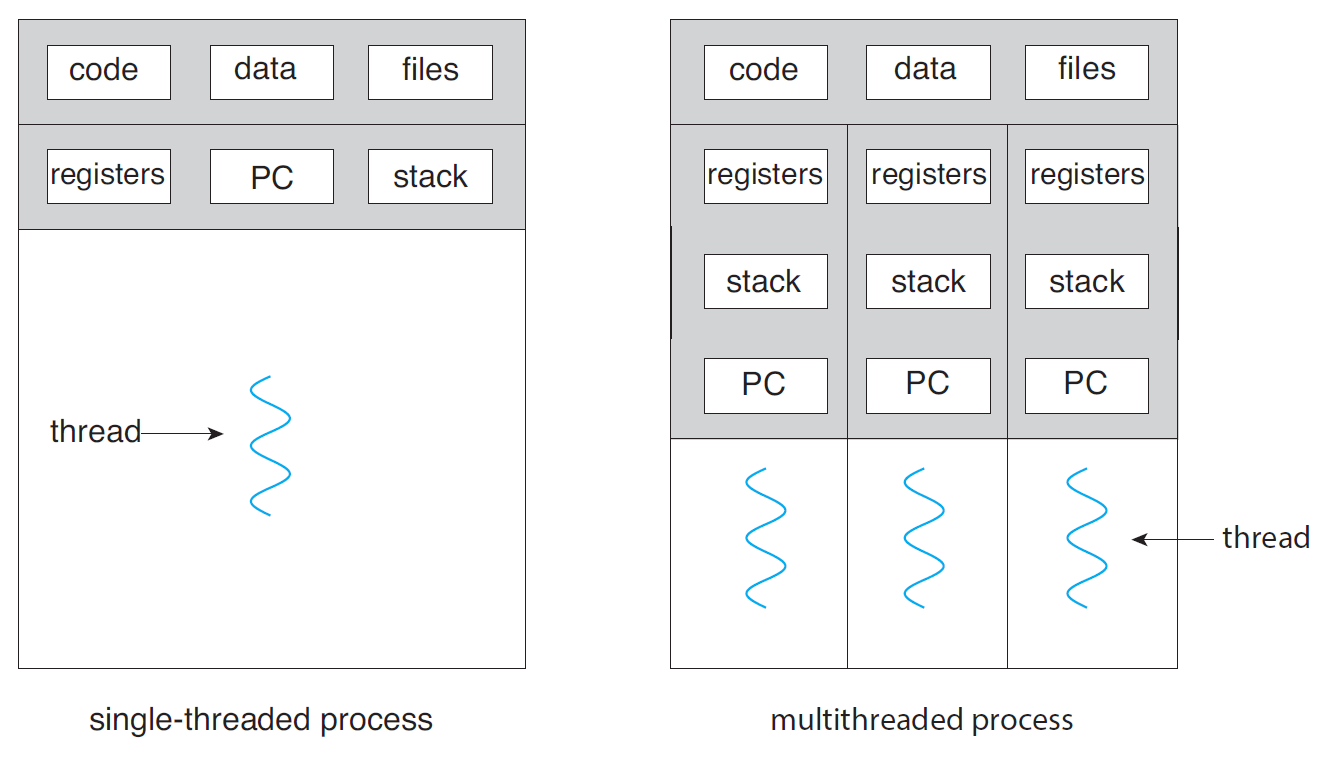
\includegraphics[keepaspectratio, width=12cm, height=9cm]{imagens/04/04 - single-multi-threaded.png}
\caption{Single and Multi-Threaded Example \\
Imagem retirada de: Silberschatz, A. Operating System Concepts, 10th,
página 160. \\}
\label{fig:imagens/04/04 - single-multi-threaded.png}
\end{figure}



O \emph{multi-threading} trás consigo diversas vantagens, como:

\begin{enumerate}
\def\labelenumi{\arabic{enumi}.}
\tightlist
\item
  Responsividade: Um programa continua rodando mesmo quando uma parte
  sua é bloqueada, trava ou demora para concluir.
\item
  Compartilhamento de Recursos: As \emph{Threads} compartilham o mesmo
  código e dados por padrão.
\item
  Economia: é mais econômico criar uma \emph{Thread} do que um processo.
  É mais rápido trocar o contexto da CPU (\emph{CPU context-switch})
  entre \emph{Threads} do que entre processos, desde que estejam em
  \emph{userspace}.
\item
  Escalabilidade: \emph{Threads} podem usufruir do paralelismo, rodando
  em múltiplas CPU's em simultâneo de forma assíncrona.
\end{enumerate}

É com o \emph{multi-threading} que um programa consegue tirar vantagem
de vários núcleos de processamento, de forma a utilizar tanto o
\emph{Concurrency} como o \emph{Parallelism} (multiplas \emph{threads}
com um único núcleo ocorre o \emph{Concurrency} mas não o
\emph{Parallelism}).

\hypertarget{funuxe7uxe3o-como-argumento-de-outra-funuxe7uxe3o.}{%
\section{Função como argumento de outra função.}\label{funuxe7uxe3o-como-argumento-de-outra-funuxe7uxe3o.}}

Utilizando Ponteiros, podemos passar uma função como argumento de outra
função, basta coletar o endereço de memória da mesma (o nome da função
coincide com o endereço dela) e passar para um ponteiro. Depois passar o
ponteiro no argumento da função. A seguir temos um código de exemplo de
como utilizar ponteiros para funções (bastando passar a variável
\texttt{fp} como argumento de uma função).



\begin{minted}[mathescape, linenos]{c}

    int funca(int); //declarando uma função sem definir
    int funcb(int);
    
    int main()
    {
            int (*fp)(int); 
            //Declarando um ponteiro de função com um argumento int
            
            fp = funca;// fp = funcb;
            printf("fp(%d) = %d\n", 3, fp(3));
    }
    
    int funca(int n)
    {
            return 2 * n
    }
    
    int funcb(int n)
    {
            return 100 * n
    }
\end{minted}



\hypertarget{complementar}{%
\section{Complementar}\label{complementar}}

\hypertarget{pesquisar-sobre}{%
\subsubsection{Pesquisar Sobre}\label{pesquisar-sobre}}

Para saber mais, procurar sobre as funções do bash \$:

\begin{enumerate}
\def\labelenumi{\arabic{enumi}.}
\tightlist
\item
  ps aux
\item
  ps aux \textbar{} wc -l
\item
  ps -ef
\item
  top (u)
\item
  htop
\item
  lscpu
\end{enumerate}

Função \texttt{C}: 1. atoi() -\textgreater{} alphabet to integer 7.